%\minisec{Graphische Dialogsysteme}
%Fenstersysteme: Applikationsfenster, Dialogfenster, Widgets

%Eingabemodell: Events (durch Tastatur/Zeigegerät)

\minisec{Ausgabemodell:}
\oitem{GeräteKoordinaten} (pixel), \\
\oitem{Geräteunabhängige Koordinaten} (z.B. in mm) wegen verschiedener Auflösungen, \\
\oitem{Weltkoordinaten:} Werte der Daten aus Modell (z.B. in Nanometern, Lichtjahren)

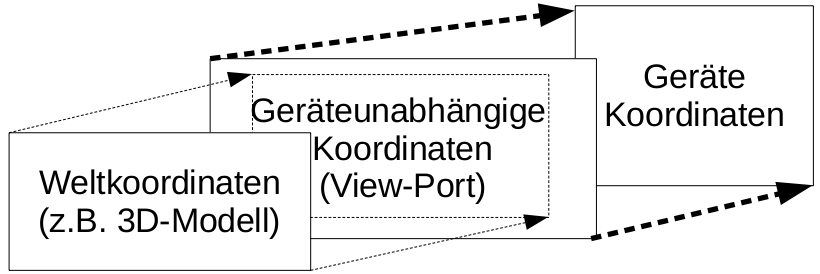
\includegraphics[width=0.25\textwidth]{ViewPort}\\
Clipping: entfernen nicht sichtbarer Objekte (Weltkoordinaten $\rightarrow$ Geräteunabhängige)\\

\minisec{Window Manager: }
Verschieben, Skalieren, Öffnen, Schließen von Fenstern,\\
Umsetzen von Platzierungsstrategien(Versuch anordung zu optimieren)\\
Bei zu großen Inhalten: Scrolling, Panning (v.A. 2D) Zooming(vgl. Google-Maps)\\

\minisec{Virtuelle Desktops:}
viel Zeit für Verwaltung der Oberfläche, zu kleine Bildschirmfläche;\\
=> Raum-Metapher: Gruppenbildung von Fenstern (Raum), wechsel zwischen Räumen\\
Alternativ: Mehr Ausgabegeräte, Previews, Fischauge,\\
ZUI (Zoomable User Interface): Detailinfos bei höheren Zoomgraden\\

\minisec{WIMP}
WIMP: Windows, Icons, Menues, Pointers\\
Post-WIMP: In nicht Bürosituationen => Ergänzen/Auflösen von WIMP\\

\begin{tabular}{|c|c|l|}
\hline
\textbf{WIMP} & \textbf{Post-WIMP}(Anti-Mac) & \textbf{Technologie} (Post)\\
\hline
Metaphor & Reality & Tangible UI\\
\hline
direct Manipulation & Delegation & Agents\\ \hline
See \& Point & Describe \& command & Natural Language UI\\ \hline
Consistency & Diversity & Bedingt durch Wechsel Ausgabegeräte \\ \hline
WYSIYG & Represent Meaning & "Letzter Versicherungsbrief" \\ \hline
User Control & Shared Control & Automatismen (z.B. Updates) \\ \hline
Feedback \&Dialog & System handles Details & Agents\\ \hline
Forgiveness & Model User actions & Planerkennung / Vorschlag Alternativen \\ \hline
Aesthetic Integrity & Graphic Variety & Bedingt durch Wechsel Ausgabegeräte  \\ \hline
Modelessness & Richer cues & Zusatzinformationen nach Verwendung \\ \hline
\end{tabular}\\


\minisec{Icons: }
Benutzerführung, ausnutzen Mustererkennung, sprachunabhängig\\
\oitem{Arten:} Repräsentativ(CD-Laufwerk), Abstrakt(Pfeile), Hybridvarianten\\
\oitem{Richtlinien:} Einfachheit/Klarheit, Verständlichkeit, Einprägsamkeit, Platzsparend, Kontrast zum Hintergrund, Unterscheidbarkeit vs Konsistenz\\
Toolbars: flexible Anordnung, konfigurierbar; meistens Sammlung von Icons


